\documentclass[10pt,a4paper]{article}
\usepackage[utf8]{inputenc}
\usepackage{amsmath}
\usepackage{amsfonts}
\usepackage{amssymb}
\usepackage{graphicx}
\usepackage{caption}
\usepackage{subcaption}
\usepackage{tabularx}
\usepackage{algorithm}
\usepackage{algcompatible}
\usepackage{listings}
\usepackage{paralist}
\usepackage{svg}
\usepackage{amsmath}
\usepackage{tikz}
\usetikzlibrary{plotmarks}
\usepackage{scrextend}
\usepackage{fourier} 
\usepackage{array}
\usepackage{makecell}
\usepackage{tabularx}
\usepackage{pbox}
\usepackage{pgfplots}
\usepackage[tableposition=top]{caption}
\usepackage[rightcaption]{sidecap}
\usepackage{graphicx} 
\graphicspath{ {images/} }


\renewcommand\theadalign{cb}
\renewcommand\theadfont{\bfseries}
\renewcommand\theadgape{\Gape[4pt]}
\renewcommand\cellgape{\Gape[4pt]}

\let\tempone\itemize
\let\temptwo\enditemize
\renewenvironment{itemize}{\tempone\addtolength{\itemsep}{-0.4\baselineskip}}{\temptwo}

\let\tempone\enumerate
\let\temptwo\endenumerate
\renewenvironment{enumerate}{\tempone\addtolength{\itemsep}{-0.4\baselineskip}}{\temptwo}

\author{Bartłomiej Zalas}
\title{System Optimization Based on Performance Evaluation Tests}

\begin{document}


\begin{titlepage}
\begin{center}


\LARGE Wrocław University of Technology\\
\large Faculty of Computer Science and Management\\[7cm]

%\begin{addmargin}[4cm]{0em}
\begin{center}
\textsc{\huge Master's Thesis}\\
\LARGE System Optimization Based on Performance Evaluation Tests \\[1.0cm]
\large Bartłomiej Zalas\\index: 192317\\[3cm]
\end{center}
%\end{addmargin}

\begin{flushright} 
\large Prepared under supervision of:\\Bogumiła Hnatkowska, Ph.D.
\end{flushright}


\vfill

% Bottom of the page
{\large Wrocław, 2017}

\end{center}
\end{titlepage}


\pagebreak
        
\tableofcontents

\pagebreak




%Content

\section{Introduction}

\subsection{Motivation}

A software optimization is the process of making software more efficient through decrease of needed resources, decrease time needed to perform certain operation by software. It can be developed on different levels of software development - source code level, algorithm optimization level, compilation level, runtime level etc. \cite{javaperformance}\cite{optimizationtheory}.

The performance evaluation tests are part of evaluation process, which is developed to ensure that software will operate correctly under desirable number of tasks in production environment \cite{analysisofpet}.   

A software optimization and a performance evaluation tests are terms related to each other. Basically, we can say that software optimization is evaluated using performance evaluation tests. 

Motivation for this work was fact that performance evaluation tests are able only to monitor performance of application. In case when application has a set of parameters influencing performance, people responsible for application performance must adjust such parameters manually or empirically. Solution able to adjust that parameters to optimize performance would be a great facilitation. 

Main goal of this work is to develop a framework, which will be able to optimize web application by search of most optimal application parameters and adjust them automatically. The first research question that needs to be answered in this work is which and how system parameters influences performance? Next, how to evaluate performance of the system? Another goal is to analyze and provide answers for question: how performance evaluation tests can help in software optimization - in monitoring and application adjustment. Another question which is emerging here is what adjustment method is the best? 

In this work author will try to consider listed problems in domain of web application optimization on runtime level using performance evaluation tests. A software under optimization and performance evaluation will be a web application simulating file storage (developed as web service) implemented in Java 1.8 Enterprise Edition and Spring Framework 1.3 deployed on Glassfish 4 server. 

\subsection{Document Structure}

//TODO


\section{Theoretical background}
Before further considerations fundamental term for this work should be defined  - a performance. 

In H. Sarojadevi's definition, performance relates to time and throughput used by application under certain workload and configuration \cite{petmethodsandtools}. In that definition workload and configuration play a role of input variables to a system/application, when time and throughput are measurable outputs from a system/application. This definition gives information about factors related to performance, but how to recognize good and bad performance?

Ian Molyneaux explains good performance as ability to use application without perceiving any delay or irritation by the end-user \cite{artperformance}. Can delay perceived by user or irritation be defined? Research \cite{howlong} shows that user expects a response from web application in about 2 seconds. Because of that there exists dependency between performance and popularity (and hence financial result) of website and that is why performance is  considered as critical for web applications from business perspective\cite{architectingperformance}. 

Knowing what is performance and how to distinguish good and bad performance one must know what indicators are used to measure performance (commonly used name for such indicator is KPI - key performance indicator). Such indicators are part of nonfunctional requirements of application in which, according to \cite{artperformance}, \cite{analysisofpet} and \cite{petmethodsandtools},  most important are:  
\begin{itemize}
\item Response time - The time needed to respond to request.
\item Throughput - The rate of requests to application.
\item Utilization - The percentage of resource usage.
\item Maximum users support - The number of concurrent users supported.
\item Workload profile - The behavior under various different amount of users.
\item Weak points - The places in which application crashes under stress conditions.
\item Scalability - The capability of a system to be enlarged to handle more amount of work.
\end{itemize}

Above indicators are used to evaluate performance of application. Process of software evaluation is called testing. G. Myers defines testing of software as a process of executing a program with the intent of finding errors \cite{arttest}. Andreas Spillner in the book "Software testing foundations" \cite{testfoundations} defines testing as execution of a application to examine it. Spillner provides also purposes of testing: 
\begin{itemize}
\item Executing a program to find failures
\item Executing a program to measure quality
\item Executing a program to provide confidence 
\item Analyzing a program or its documentation to prevent failures
\end{itemize}

All four purposes are applicable in performance evaluation tests - failures are found when application does not behave as it is designed under given workload, application quality and performance capabilities are measured, confidence that application will serve desired amount of requests is provided, analysis of bottlenecks helps to improve system. 

At the same time we need to have in mind Edsger W. Dijkstra's sentence:
testing shows the presence, not the absence of bugs \cite{set}. That's why  software tests should cover possibly largest set of application use scenarios.  

The test to see whether the application meets documented performance specifications (KPIs) is called performance evaluation test \cite{arttest}. 
In order to process performance evaluation tests a set of activities must be performed. According to Ian Molyneaux \cite{artperformance} following steps should be performed:
\begin{itemize}
\item Nonfunctional Requirements Capture - definition of performance target, performance testing schedule, environment design.
\item Performance Test Environment Build - deployment of the application, configuration and deployment of testing tools and KPI monitoring.
\item Use-Case Scripting - input data requirements, selection of areas to monitor for response time, ensure of correctness or use case replays.
\item Performance Test Scenario Build - creation of test scenarios, and realistic throughput model
\item Performance Test Execution and Analysis - execution of tests and results analysis.
\item Post-Test Analysis and Reporting - collection and analyze of  data from all test runs, reports creation.
\end{itemize}

Accordingly to our objectives different kinds of performance tests may be carry out. In the literature \cite{artperformance},\cite{architectingperformance} and \cite{analysisofpet} three main types of performance testing can be found:
\begin{itemize}
 \item Load testing - To validate application behavior under normal and peak conditions.
 \item Stress testing - To validate application behavior beyond normal load conditions.
 \item Capacity testing - To find a limits of users and transactions which an application is able to handle.
\end{itemize}

Performance evaluation tests can be done manually (by testers playing role of an end user \cite{comparison}) or automatically (using tools which are able to perform workload simulation, monitor indicators and generate reports). Manually testing in most of the cases is time consuming, expensive and hectic. For the better business purpose and to save time and money automation testing is required \cite{automaiontools}.

Examples of automated performance testing tools are: Selenium \cite{automaiontools}, Apache JMeter, NeoLoad, LoadRunner and others \cite{analysisofpet}. Common features offered by this tools are \cite{analysisofpet}: 
\begin{itemize}
 \item Heavy load simulation;
 \item Measuring and monitoring performance indicators;
 \item Performance report generation;
 \item Possibility to customize tests by scripts/API;
\end{itemize}

Most important features of automated performance evaluation tests are repeatability (each time application is under the same workload) and autonomy (human role in testing process is limited only to start tests and analyse results). These features give possibility to conduct performance evaluation tests frequently during development phase or can be even included to continuous integration process. Such approach would deliver (practically) instant feedback for developers about impact of new created features on performance \cite{autobugs}. 

Other important features, defined by Molyneaux, which should be considered during choosing testing tool are:
\begin{itemize}
 \item Protocol support - communication between an application and a testing tool
 \item Licensing model - pricing and cost
 \item Scripting effort - manual script changes to reply tests
 \item In-house versus outsourced - way of hosting performance testing tools.
\end{itemize}

Knowing what is performance, how is measured and how to develop environment for performance evaluation and tests itself, next important step is optimization of application. 

Singiresu Rao defines optimisation as the act of obtaining the best result under given circumstances \cite{optimizationtheory}. In performance oriented development and testing, as in this work, "best result" can be understood as best performance (measured as execution time and resources consumption). "Given circumstances" can be interpreted as workload, current software environment configuration and correctness of chosen algorithms and implementation decisions in an application. 

According to  \cite{javaperformance} software optimization for Java environment can be achieved at many areas, like: compiler optimization, garbage collector tuning, heap memory customization, optimal memory management, threads control, database queries optimization, JVM adjustment, and others.

For the web applications specific types of optimization can be performed.  
The book "Architecting High Performing, Scalable and Available Enterprise Web Applications"  provides information about elements which should be used to optimize web application. This elements are \cite{architectingperformance}:
\begin{itemize}
 \item HTML optimization - usage of HTML 5 and CSS 3 performance features such as application cache, web SQL, web sockets, CPU optimization. This features should be considered and introduced during application development; 
 \item high performance responsive web design - used to automatically adjust content of a web page to browser resolution; 
 \item assets optimization - images, videos, JavaScript files, style sheets should be compressed and minimized; 
 \item proper cache configuration - when requested, server should response with new content of resource only when it was changed from the last request, otherwise "Not Modified" (304) should be returned;
 \item CDN accelerators - geographically distributed servers accelerating  load of web page assets; 
 \item asynchronous and on-demand rendering - web page architecture where only demanded regions of page are rerendered after user actions.  
\end{itemize}

Above elements are related to client side and are responsible for data presentation and user experience. They should be taken into consideration during application development and deployment. Because are not configurable during application runtime and do not influence application core performance, which is responsible for serving data to client side are out of scope of this work. 

\section{Existing Topics Related to Software Performance}

\subsection{Performance Related Problems} \label{PerformanceRelatedProblems}
One of the most fundamental problem about applications performance is a nasty habit of turning up late in the application life cycle \cite{artperformance}. In article "Performance Anti-Patterns" \cite{lssrarticle} Bart Smaalders noticed that development teams overloaded by new features development and bug fixing left performance work as an afterthought. The first report from performance is received from developed software versions during beta testing.

To solve and avoid above problem, performance evaluation tests should be repeatable, observable, portable, easily presented, realistic, runnable. Thanks to that tests can be executed as early as possible during software development cycle, and executed continuously during development providing instant performance feedback to the developers. 

Another problem with web applications served in enterprise environment is multiplicity of manual configuration of parameters needed to create optimal environment for application. Table \ref{glassfishparams} presents common parameters influencing performance of Java application server \cite{glassfishdoc} \cite{deployerproblem}.  

\begin{table}[!htb]
\caption{\textit{Common Java application server parameters influencing performance.}}
\def\arraystretch{1.5}
\begin{tabularx}{\textwidth}{l|X}
  \textbf{Parameter} & \textbf{Performance Influence} \\
\hline
Max Thread Pool Size & Increasing this value will reduce HTTP response latency times but may also overload CPU.\\
 
Data Connection Pool Size & Small connection pool has faster access on the connection table, but requests may spend more time in the queue. Large connection pool requests will spend less (or no) time in the 
queue, but access on the connection table is slower.\\

EJB Pool Size & Large pool wastes memory and  can slow down the system. A very small pool is also inefficient due to contention. \\

JVM Heap Size & Increasing heap size can improve performance, but too high memory usage by JVM can slow down a system.   \\

JVM GC Algorithm & Available algorithms have different influence on pause 
times, throughput and CPU usage.
\end{tabularx}
\label{glassfishparams}
\end{table}

In article "The deployer's problem: configuring application servers for performance and reliability" \cite{deployerproblem} authors provide method for finding good configuration for the application deployment:

\begin{enumerate}
\item For each configuration value of interest, select a reasonable range. 
\item Generate random value from range
\item Deploy application with chosen value
\item Measure performance
\item Repeat steps 2-4 until performance of application is satisfying. 
\end{enumerate}

Presented procedure is obviously time consuming - requires manual parameter tuning and application deployment - and deficient because of random parameters value selection. This disadvantages show need of automated tool which will be able to automatically perform above steps and choose the best configuration.

The web applications are characterised by various workload. Such characteristic is dependent from profile and purpose of web application \cite{invariantsworkloads}. This fact should be also taken into consideration during tuning application performance. 

\subsection{Existing solutions} \label{ExistingSolutions}
In article "Automatic Performance Tuning for J2EE Application Server Systems" \cite{autotuning} authors proposed a solution for automatic application optimization based on \textit{MaxPoolSize} parameter of JBoss application server resulting in 37\% improvement. What is also important, proposed dynamic configuration  mechanism  was able to improve  performance  and  adapt  to  changes  in  workloads without human intervention. In the article authors also noticed that there is no fully automated framework designed for Java Enterprise application server reconfiguration.

General idea of self-optimization systems was proposed in the article "The Vision of Autonomic Computing" \cite{autoarch}. Main problem introduced by authors is complexity and great number of tunable parameters influencing performance. Also, tuning of one subsystem can have unanticipated effects on the entire system. Proposed solution is Autonomic system. System which will continually seek ways to improve their operation, identifying and seizing opportunities to make themselves more efficient in performance or cost. 

A framework for automatic performance tuning is presented in article "Automatic Performance Management in Component Based Software Systems" \cite{autoframework}. The framework consist of two main modules: monitoring and diagnostic module and application adaptation module. The monitoring and diagnostic part gathers data about performance of application and environment with minimal overhead. Informations about probes (performance data related to method execution and lifecycle
events of EJB) are analyzed and in case of performance problems alert is raised. When it happens, application module should overcome performance problems by selecting software component which will provide the best possible performance at given run-time context. 

Such concept is called component redundancy and is described deeper in the article "A framework for using component redundancy for self-adapting and self-optimising component-based enterprise systems" \cite{redundancycomponent}. In the article author describes Component Redundancy as presence, at runtime, of multiple  component  variants  providing  identical or equivalent services but with different implementation strategies. Only one of the redundant components providing a service is assigned, at any moment in time, for handling a certain client request for that  service.  Implementation strategies can be added or deleted during runtime. Depending from context (workload, available resources) suitable component is selected. Selection is based on component description - set of attributes which defines in what conditions component usage is the most optimal. These descriptions are then updated at runtime with accurate monitoring information for the actual execution contexts. 

The practical approach of software performance optimization from implementation level is described in book "Pro Spring 2.5" in chapter "Spring Performance Tuning" \cite{springperformance}. In this chapter authors present most typical performance related problems and explain how to analyze performance and how to find bottlenecks of application written in Spring Framework. Key indicator in presented process is execution time of a method. Major part of text is focused on improving the data access tier by following improvements:  
\begin{itemize}
\item paged data - records from database are queried in chunks, 
\item lazy loading - only records requested by user are returned from query (without related tables), 
\item indexing - database index are created in order to improve search, 
\item batched inserts - records are inserted/updated into database in chucks
\end{itemize}
In the book, authors provide guide how to increase performance in other areas:
\begin{itemize}
\item view performance - fast rendering of web page
\item cache - basic usage of method cache is presented
\end{itemize}
The text provides examples with source code. The authors of the book emphasize that each performance improvement should be based on understanding bottleneck and be adapted to application and users profile.  

\subsection{Summary}

In section \ref{PerformanceRelatedProblems} problems related to software optimization and performance evaluation tests where presented. Conclusion in the form of list presented below shows main raised problems:
\begin{itemize} 
\item Downplaying of performance evaluation tests \cite{artperformance}\cite{lssrarticle}
\item Complexity of performance tuning \cite{glassfishdoc}\cite{deployerproblem}
\item Process of performance tuning is time consuming and manual \cite{deployerproblem}
\item Workload (number of requests to an application) is various \cite{invariantsworkloads}
\end{itemize}

Analysis of existing problems from section \ref{ExistingSolutions} provides also solutions, ideas and hints addressing above problems:
automatic performance tuning \cite{autotuning}\cite{autoarch}\cite{autoframework}, redundant components \cite{redundancycomponent} and suitable implementation decisions \cite{springperformance}. 

Automatic performance tuning addresses problem with time consuming and complex configuration. Due to fact that application performance is monitored continuously such tuning is performed instantly when needed. Next advantage of such system is that it knows how to achieve the best performance in given circumstances. 

The idea of redundant component gives possibility to develop solution which will fit well to changeable environment. Managed by automatic performance tuning system may be switched during runtime when system usage characteristic change. 

Suitable performance related decisions impose on developers duty to awareness of performance influence of taken implementation decisions. Developers should be aware of system workload characteristic in production environment and perform performance optimization where possible. 
 
\section{Proposed solution}

\subsection{About This Chapter}
On the base of previous chapters author of this work will try to provide solution which will be addressing most of listed problems from chapter \ref{PerformanceRelatedProblems}. Next subsections provide considerations about possible ways to obtain the best possible solutions with justification. Final goal is to implement system which will demonstrate and evaluate implemented solutions. 

\subsection{Tested application}  
As mentioned in previous chapters performance optimization can be developed in many areas. For this work author will focus on web based application. The application will be a service simulating product database - basic CRUD operations on products categories will be provided. Details about entities managed by tested application are presented on Figure \ref{erd}. 

\begin{figure}[h]
\centering
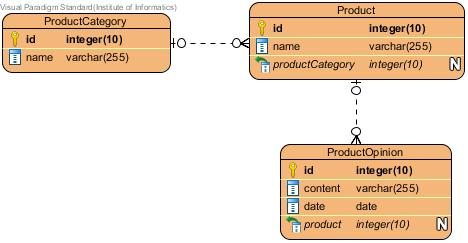
\includegraphics[width=0.6\textwidth]{erd}
\caption{\textit{ERD diagram of tested application model}}
\label{erd}
\end{figure}

For simplicity and in order to concentrate on the topic of this work graphical user interface will be omitted. Communication with application will be provided in form of REST service. Provided REST API is presented in the Table \ref{restapi}.

\begin{table}[!htb]
\def\arraystretch{1.5}
\caption{\textit{Tested application REST API}}\label{restapi}
\begin{tabularx}{\textwidth}{p{2cm}|p{1.2cm}|X|p{2cm}}
  \textbf{Path} &\textbf{Method} & \textbf{Parameters} & \textbf{Produces} \\
  \hline
  addCategories & PUT & - & String \\ 
  findAll & GET & - & JSON\\
  findPart & GET & page:Integer, size:Integer & JSON\\
  findById & GET & id:Integer, & JSON \\
  updateById & POST & id: Integer, newName:String & JSON \\
  add & PUT & categoryName:String & String\\
\end{tabularx}
\end{table}


The application will be developed in Java language using Spring Framework. The application server for the application will be Apache Tomcat served by Spring Bootstrap 1.5. Data persistence will be realized in PostgreSQL 9.6 DBMS.  

\subsection{System Principles}
The key in every successful project is to define goals and needs at the beginning.
In case of this work it will be realized as system principles definition on the base of  performance problems from chapter \ref{PerformanceRelatedProblems}.

Downplaying of performance evaluation tests - decision of when, how often or even if perform performance evaluation tests lays in developers way of working. However, performance evaluation tests performed in easy way with minimal effort could encourage developer teams to perform it. 

Complexity of performance tuning - the system should know which set of configuration parameters values will be the best in given situation.  

Process of performance tuning is time consuming and manual - the system should know how to tune configuration to increase performance of application and do it automatically. 

Workload is various - the system should be able to monitor workload of application in form of incoming requests in order to switch application configuration which will be more suitable in given circumstances. 

On the base of above consideration following set of principles of the system can be formulated:

\begin{itemize}
\item The system should perform live monitoring of application
\item The system should be autonomous
\item The system should be able to perform configuration change during application runtime
\item The system should be able to work in production environment
\item The system should have minimal impact on production environment
\end{itemize}

On the base of above principles in next chapter proposition of system realization will be introduced.  

\subsection{Performance Improvement Realization}

Before system architecture will be introduced a set of elements on which performance tuning will be performed must be introduced.  
Considering existing solutions presented in chapter \ref{ExistingSolutions} author of this work decided to perform performance tuning of the application on the base of two techniques: redundant components and application server configuration parameters. 

\subsubsection{Redundant Components}
Redundant components, by definition, provide the same services but with different implementation. From the performance perspective that idea can be used to implement component which will provide the same services with different performance characteristic. What is also important, usage of redundant components must be justified - there must exist circumstance where given redundant component will offer better performance than another redundant component. 

Author of this work decided to took into consideration following candidates: paging, cache, batched inputs. The decision was based on facts that all of mentioned candidates are able to increase performance of the  tested application domain and it is possible to develop a switchable equivalent for given a candidate. 

Paging is database query realization in which in a single select query only part (page) of records is returned instead of querying all records from database. Table \ref{pagingcomponents} shows comparison of two proposed redundant components: Paging and No Paging.  
\begin{table}[!htb]
\def\arraystretch{1.5}
\caption{\textit{Paging redundant components comparision}}\label{pagingcomponents}
\begin{tabularx}{\textwidth}{p{3cm}|X|X}
  \textbf{Category} &\textbf{Paging} & \textbf{No Paging} \\
\hline
Query all records & Multiple queries (slower) & One query (faster) \\
User satisfaction & High & Low\\
Top performance circumstances & When impossible to query all records by No Paging component & When possible to query all records at once\\
\end{tabularx}
\end{table}

\begin{figure}[!htb]
\centering
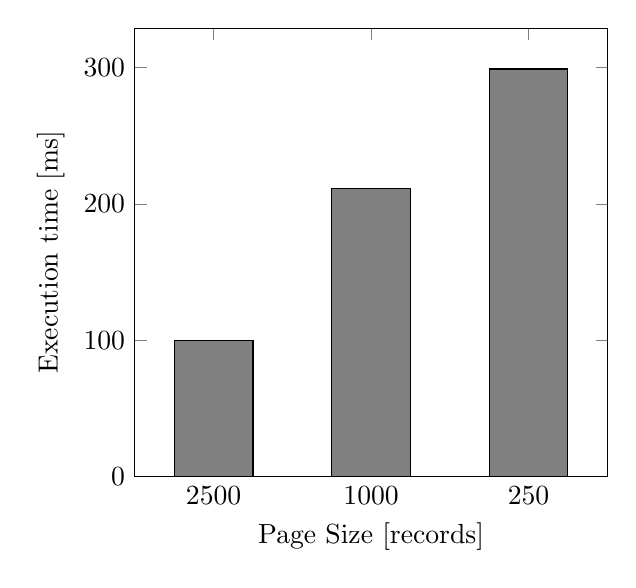
\begin{tikzpicture}
        \begin{axis}[
            symbolic x coords={{2500}, {1000}, {250}},
            xtick=data,
            bar width=1cm,
            x=2cm,
            ymin=0,
            enlarge x limits={abs=1cm},
            xlabel={Page Size [records]},
            ylabel={Execution time [ms]}
          ]
            \addplot[ybar,fill=gray] coordinates {
                ({2500},  100)
                ({1000},  211)
                ({250},   299)
            };
        \end{axis}
\end{tikzpicture}
\caption{\textit{Execution time comparision for different page size for 10000 records}} \label{fig:pagesizetime}
\end{figure}

As shown in Figure \ref{fig:pagesizetime} the bigger page size is, the smaller execution time is. It is related to fact that every query to a database generates additional overhead. 
In general the No Paging component is faster when it is possible to query all records at once. Possible to query means that query will not need more resources (memory, CPU) than is needed to be performed. 
The Paging component must perform multiple queries to a database in order to query all existing records. From the practical point of view in presentation layer only first page of records is needed when user entering a web page. Otherwise, long time of No Paging component execution will decrease user satisfaction level.  

The paging idea is more related to data presentation layer and user satisfaction. Moreover, when number of records in a database is possible to query at once No Paging component will be always faster to query all records. Because of that author of this work decided to reject paging as redundant component. 

Next redundant component candidate is cache. There exist many levels of abstraction on which cache can be applied to a web application - request level cache, method level cache, global data cache. For goals of this work method-level cache of service responsible for managing database operations was chosen - in general such operations are time consuming. The cache saves returned value from method and uses input parameters as cache key. Table \ref{cachecomponents} shows comparison of two proposed redundant components: Cache (methods are cached) and No Cache (cache is disabled).
\begin{table}[!htb]
\def\arraystretch{1.5}
\caption{\textit{Cache and No Cache redundant components comparision.}}\label{cachecomponents}
\begin{tabularx}{\textwidth}{p{3cm}|X|X}
  \textbf{Category} &\textbf{Cache} & \textbf{No Cache} \\
\hline
Preferable parameters characteristic & Repeatable & Varied \\
Preferable resources & Immutable & Mutable\\
Overhead & Yes & No\\
\end{tabularx}
\end{table}
 
Table \ref{cachecomponents} shows that Cache and No Cache redundant components have different characteristic. In workload in which requests are repeatable (given set of parameters is used more than once) and there are no frequent changes in state of requested resources (no updates and inserts into a database) preferred redundant component is Cache. When there is no repeatable requests and requested resources are frequently changed, usage of cache generates only additional overhead. In such cache No Cache component should be used. On the base of above considerations Cache/No Cache components could be considered as a proper redundant component from performance perspective and will be implemented in the system. 

Last redundant component taken into consideration are batched inserts. The idea is to gather objects which are to be inserted into a database and insert them in one query instead of few separate ones. This minimize query overhead. In case of this work inserts batch is realized in form of collection of the objects in which insert query is fired when collection is full.   
Table \ref{batchedcomponents} shows comparison of two proposed redundant components: Batched (records to insert are batched) and Direct (direct inserts into a database as separate queries).

\begin{table}[!htb]
\def\arraystretch{1.5}
\caption{\textit{Paging redundant components comparision.}}\label{batchedcomponents}
\begin{tabularx}{\textwidth}{p{3cm}|X|X}
  \textbf{Category} &\textbf{Batched} & \textbf{No Batched} \\
\hline
Query execution time & Faster & Slower \\
Query effects & Delayed & Instant\\
Efficiency & High & Low\\
\end{tabularx}
\end{table}

\begin{figure}[!htb]
\centering
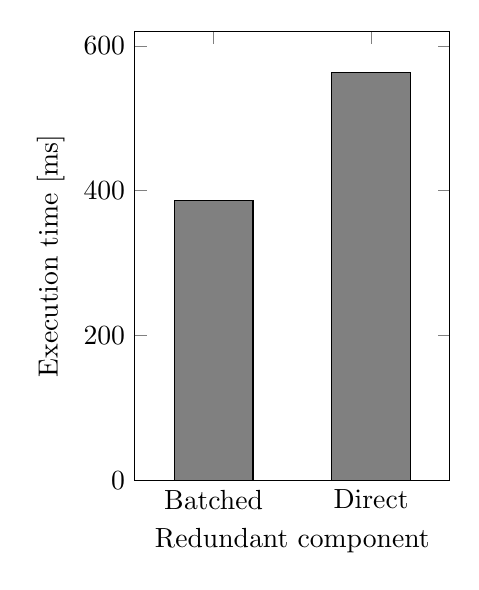
\begin{tikzpicture}
        \begin{axis}[
            symbolic x coords={Batched, Direct},
            xtick=data,
            bar width=1cm,
            x=2cm,
            ymin=0,
            enlarge x limits={abs=1cm},
            xlabel={Redundant component},
            ylabel={Execution time [ms]}
          ]
            \addplot[ybar,fill=gray] coordinates {
                (Batched,  386)
                (Direct,   563)
            };
        \end{axis}
\end{tikzpicture}
\caption{\textit{Execution time comparision for Batched and Direct redundant components for batch with size = 10 and 20 inserted records}} \label{fig:batchedtime}
\end{figure}

The components comparison in Table \ref{batchedcomponents} shows different characteristic of both redundant components. Batched one is in general more efficient and faster than No Batched. However, process of batching records introduces delays in real effect of batched statement (equal to time in which given records sf "frozen" in the batch). In proposed implementation batched statement will be fired when batch is full. Both facts lead to conclusion that Batched component should be used only in circumstances when such delay is acceptable by users or when number of inserts into a database is so high that efficiency improvement is needed. Another thing is the more frequent inserts into a database (faster filling up of batch) the smaller delay. Therefore Batched component should be used only in case when number of inserts into a database is very high. Otherwise Direct component should be used. Above considerations justify choice of Batched/Direct redundant components to be used in the system.   

\subsubsection{Application Server Configuration Parameters}

Configuration of application server is crucial in performance of application. Application servers provide wast number of parameters which can be configured. Such parameters may be slightly different depending from vendor but in most cases configuration provide possibility to adjust: thread number, JDBC connection pools, EJB pools, JVM configuration. 

Author of this work decided to take into consideration 2 possible configurations: EJB pool size and thread number of application server. Both configurations have direct influence on number of requests which are handled by application and should provide high performance improvements in the application domain. 

EJB pooling mechanism reduces time needed for creating new bean instances (beans are created on start up and kept in pool) and support parallel request handling. In case of this work tested application is developed in Spring framework in which all beans are singletons by default. Therefore EJB pool configuration has no effect on application performance. Influence of EJB pool size on performance of enterprise application was used up in other work \cite{autotuning} where authors already proved that tuning EJB pool size has positive influence on a JEE application performance. Taking into account this arguments EJB pool will be not implemented in the system. 

Number of threads has key meaning in handling incoming requests into an application server. When number of threads is less than parallel incoming requests not handled part will be waiting in the queue until threads will be free again. Too large number of threads results in increased CPU usage and slower performance. This fact is documented in the Figure \ref{fig:threads}. For 100 incoming parallel requests tested 3 configuration of thread number: 10 threads, 200 threads, 10000 threads. As one can see the worst mean response time was when number of threads was smaller than number of requests. Too high number of threads also negatively influences performance.   

\begin{figure}[!htb]
\centering
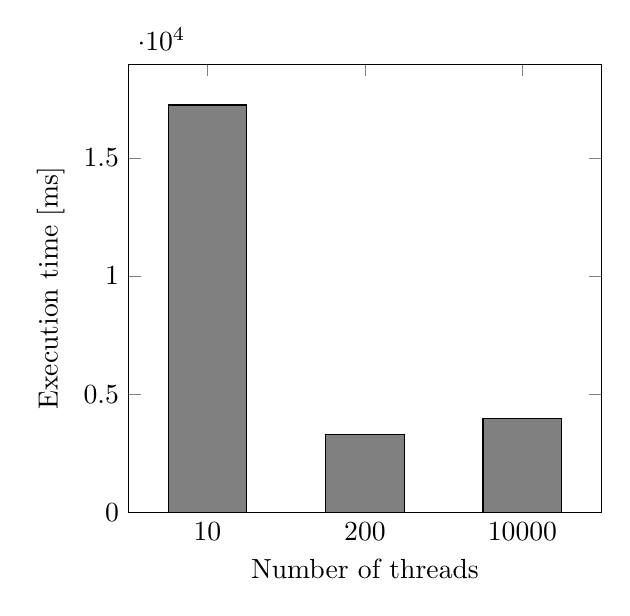
\begin{tikzpicture}
        \begin{axis}[
            symbolic x coords={10, 200, 10000},
            xtick=data,
            bar width=1cm,
            x=2cm,
            ymin=0,
            enlarge x limits={abs=1cm},
            xlabel={Number of threads},
            ylabel={Execution time [ms]}
          ]
            \addplot[ybar,fill=gray] coordinates {
                (10,  17236)
                (200,   3296)
                (10000,   3963)
            };
        \end{axis}
\end{tikzpicture}
\caption{\textit{Mean response time from 100 incoming paraller requests}} \label{fig:threads}
\end{figure}

Number of threads has large impact on application performance and it configuration will be implemented in the system. 

\subsubsection{Performance Improvement Realization Summary}

Above considerations contain justification about accepted or declined candidates for performance tuning in the system. Finally, two redundant components (batched imports, cached methods) and one application server configuration parameter (threads number) was chosen.


\subsection{The System Architecture}
...



\pagebreak

\section{References}
\renewcommand\refname{}
\begin{thebibliography}{9}

\bibitem{artperformance}
Molyneaux I., 
\textit{The Art of Application Performance Testing}, 
Sebastopol USA, O’Reilly Media, 2015.

\bibitem{javaperformance}
Oaks S., 
\textit{Java Performance: The Definitive Guide}, 
Sebastopol USA, O’Reilly Media, 2014.

\bibitem{optimizationtheory}
Rao S. S., 
\textit{Engineering Optimization Theory and Practice}, 
New Jersey USA, John Wiley \& Sons, Inc., 2009.

\bibitem{lssrarticle}
Smaalders B., 
\textit{Performance Anti-Patterns},
Queue, New York USA, vol. 4, no. 1, 2006

\bibitem{architectingperformance}
Kumar Shivakumar S. K. , 
\textit{Architecting High Performing, Scalable and Available Enterprise Web Applications},
Waltham USA, Elsevier, 2015, 101-141.

\bibitem{idealvalues}
Patel C. , Gulati R., 
\textit{Identifying Ideal Values of Parameters for Software Performance Testing},
IEEE, 2015 International Conference on Computing, Communication and Security (ICCCS), 4-5 Dec. 2015

\bibitem{comparison}
Kaur M., Kumari R.,
\textit{Comparative Study of Automated Testing Tools: TestComplete and QuickTest Pro},
International Journal of Computer Applications (0975 – 8887) Volume 24 - No.1, June 2011

\bibitem{analysisofpet}
Sharmila S., Ramadevi E.,
\textit{Analysis of Performance Testing on Web Applications},
International Journal of Advanced Research in Computer and Communication Engineering Vol. 3, Issue 3, March 2014

\bibitem{petmethodsandtools}
Sarojadevi H.,
\textit{Performance Testing: Methodologies and Tools}
Journal of Information Engineering and Applications, Vol 1, No.5, 2011.

\bibitem{howlong}
Fui-hoon F.,
\textit{A study on tolerable waiting time: how long are Web users willing to wait?}, Behaviour \& Information Technology, 23:3, 153-163, February 2007.

\bibitem{howlong}
Dang Q., Ignat C., 
\textit{Performance Evaluation of Web Based Automation Testing Tools}, Behaviour \& Information Technology, 23:3, 153-163, February 2007.

\bibitem{automaiontools}
Angmo R., Sharma M., 
\textit{Performance evaluation of web based automation testing tools}, 
5th International Conference - Confluence The Next Generation Information Technology Summit (Confluence), Noida, 2014, pp. 731-735.

\bibitem{autobugs}
Tsakiltsidis S., Miranskyy A., Mazzawi E., 
\textit{On Automatic Detection of Performance Bugs},
IEEE International Symposium on Software Reliability Engineering Workshops (ISSREW), Ottawa, ON, Canada, 2016, pp. 132-139.

\bibitem{arttest}
Myers G. J. , Sandler C.,  Badgett T.,
\textit{The art of software testing, Third Edition},
Hoboken, New Jersey, USA, John Wiley \& Sons, Inc., 2012

\bibitem{testfoundations}
Spillner A., Linz T., Schaefer H.,
\textit{Software testing foundations, Fourth Edition},
Sebastopol, California, USA, O‘Reilly Media, 2014

\bibitem{set}
Buxton J.N.,Randell  B., 
\textit{Software Engineering Techniques}, 
Rome, Italy, Report on a conference sponsored by the NATO Science Committee, p. 16., 1970

\bibitem{glassfishdoc}
\textit{GlassFish Server Open Source Edition, Performance Tuning Guide}, 
https://glassfish.java.net/docs/4.0/performance-tuning-guide.pdf,
Oracle, May 2013

\bibitem{deployerproblem}
Raghavachari M., Reimer D., Johnson R. D., 
\textit{The deployer's problem: configuring application servers for performance and reliability}, 
25th International Conference on Software Engineering, 2003. Proceedings.,2003, pp. 484-489.

\bibitem{invariantsworkloads}
Menascé D. A., Almeida V. A. F., Riedi R., Pelegrinelli F., Fonseca R., Meira W.,  
\textit{In Search of Invariants for E-Business Workloads} 
In Proceeding of Second ACM Conference on Electronic Commerce, Minneapolis, October 17-20, 2000. 

\bibitem{autotuning}
Zhang Y., Qu W., Liu A., 
\textit{Automatic Performance Tuning for J2EE Application Server Systems.}  Web Information Systems Engineering. WISE 2005. Lecture Notes in Computer Science, vol 3806. Springer, Berlin, Heidelberg

\bibitem{autoarch}
Kephart J. O., Chess D. M., 
\textit{The vision of autonomic computing}, in Computer, vol. 36, no. 1, pp. 41-50, Jan 2003.

\bibitem{autoframework}
Diaconescu A., Mos A., Murphy J., \textit{Automatic performance management in component based software systems}, International Conference on Autonomic Computing, 2004. Proceedings., 2004, pp. 214-221.

\bibitem{redundancycomponent}
Diaconescu A., \textit{A framework for using component redundancy for self-adapting and self-optimising component-based enterprise systems}, 2003, In Companion of the 18th annual ACM SIGPLAN conference on Object-oriented programming, systems, languages, and applications (OOPSLA '03). ACM, New York, NY, USA, 390-391. 

\bibitem{springperformance}
Chakraborty, A., Ditt, J., Vukotic, A., Machacek, J., \textit{Pro Spring 2.5}, Berkeley, CA, Apress, 2008, 829-855,  


\end{thebibliography}


\end{document}
